\documentclass[a4paper,11pt]{article}
\usepackage[utf8]{inputenc}
\usepackage[T1]{fontenc}
\usepackage{geometry}
\usepackage{enumitem}
\usepackage{titlesec}
\usepackage[table]{xcolor}
\usepackage{fancyhdr}
\usepackage{tikz}
\usetikzlibrary{shapes.geometric, arrows, positioning, fit, backgrounds}
\usepackage{tabularx}
\usepackage{listings}
\usepackage{graphicx}
\usepackage{lastpage}
\usepackage{hyperref}

% Page Setup
\geometry{top=1in, bottom=1in, left=0.8in, right=0.8in}
\pagestyle{fancy}
\fancyhf{}
\lhead{\small Project 83: Agentic AI Compiler Assistant}
\rhead{\small Week 4 Report}
\cfoot{\thepage\ of \pageref{LastPage}}

% Formatting
\titleformat{\section}{\Large\bfseries\color{blue!70!black}}{\thesection.}{1em}{}[\titlerule]
\titleformat{\subsection}{\large\bfseries\color{blue!50!black}}{\thesubsection}{1em}{}

% Code Listings Configuration
\lstset{
    basicstyle=\ttfamily\small,
    breaklines=true,
    frame=single,
    backgroundcolor=\color{gray!10},
    keywordstyle=\color{blue},
    stringstyle=\color{green!50!black},
    commentstyle=\color{gray},
    showstringspaces=false,
    tabsize=4,
    captionpos=b
}

% Custom commands
\newcommand{\statusgood}[1]{\colorbox{green!20}{\textbf{#1}}}
\newcommand{\statuspending}[1]{\colorbox{yellow!20}{\textbf{#1}}}
\newcommand{\statusissue}[1]{\colorbox{red!20}{\textbf{#1}}}

% TikZ styles for architecture diagrams
\tikzstyle{component} = [rectangle, rounded corners, minimum width=3cm, minimum height=1cm, text centered, draw=black, fill=blue!20]
\tikzstyle{interface} = [rectangle, minimum width=3cm, minimum height=0.8cm, text centered, draw=black, fill=green!20]
\tikzstyle{arrow} = [thick,->,>=stealth]
\tikzstyle{bidiarrow} = [thick,<->,>=stealth]
\tikzstyle{layer} = [rectangle, draw=black, thick, dashed, inner sep=10pt]

\begin{document}

\begin{center}
    {\huge \textbf{Week 4 Progress Report}} \\
    \vspace{3mm}
    {\large \textbf{Project 83: Conversational Agentic AI Compiler Assistant}} \\
    \vspace{2mm}
    \textit{System Architecture \& Technical Design Specification} \\
    \vspace{2mm}
    \textbf{Reporting Period:} Week 4 | \textbf{Status:} \statusgood{COMPLETED}
\end{center}

\vspace{5mm}

\section{Executive Summary}

Week 4 represented a critical transition from requirements analysis to detailed technical design, establishing the architectural foundation for the entire Agentic AI Compiler Assistant system. This week focused on bridging traditional compiler theory with modern AI-powered assistance through a carefully designed, modular architecture.

\textbf{Key Achievement:} Successfully designed a comprehensive multi-layered architecture that cleanly separates compiler components (Lexer, Parser, Semantic Analyzer, Code Generator) from AI orchestration layers while maintaining extensibility and modularity. Created detailed architectural diagrams including system overview, component interactions, and data flow visualizations.

\subsection{Week Overview}

\begin{itemize}[leftmargin=*]
    \item \textbf{Planned Objectives:} System architecture design, UML diagrams, class-level structure definition
    \item \textbf{Achieved Objectives:} Complete layered architecture, Compiler-Agent Bridge specification, orchestration workflows, 5 architectural diagrams
    \item \textbf{Completion Rate:} 100\%
    \item \textbf{Documentation:} 45 pages of architectural specifications
\end{itemize}

\section{System Architecture Overview}

\subsection{2.1 Architectural Principles}

The system architecture adheres to the following fundamental principles:

\begin{enumerate}
    \item \textbf{Separation of Concerns:} Clear boundaries between compiler pipeline phases and AI orchestration components
    \item \textbf{Modularity:} Each component can be developed, tested, and deployed independently
    \item \textbf{Extensibility:} Architecture supports adding new compiler phases or AI agents without major refactoring
    \item \textbf{Maintainability:} Well-defined interfaces and data contracts between components
    \item \textbf{Testability:} Each layer can be tested in isolation with mock dependencies
    \item \textbf{Performance:} Asynchronous processing for AI calls to avoid blocking compiler pipeline
\end{enumerate}

\subsection{2.2 High-Level Architecture Diagram}

\begin{figure}[h]
\centering
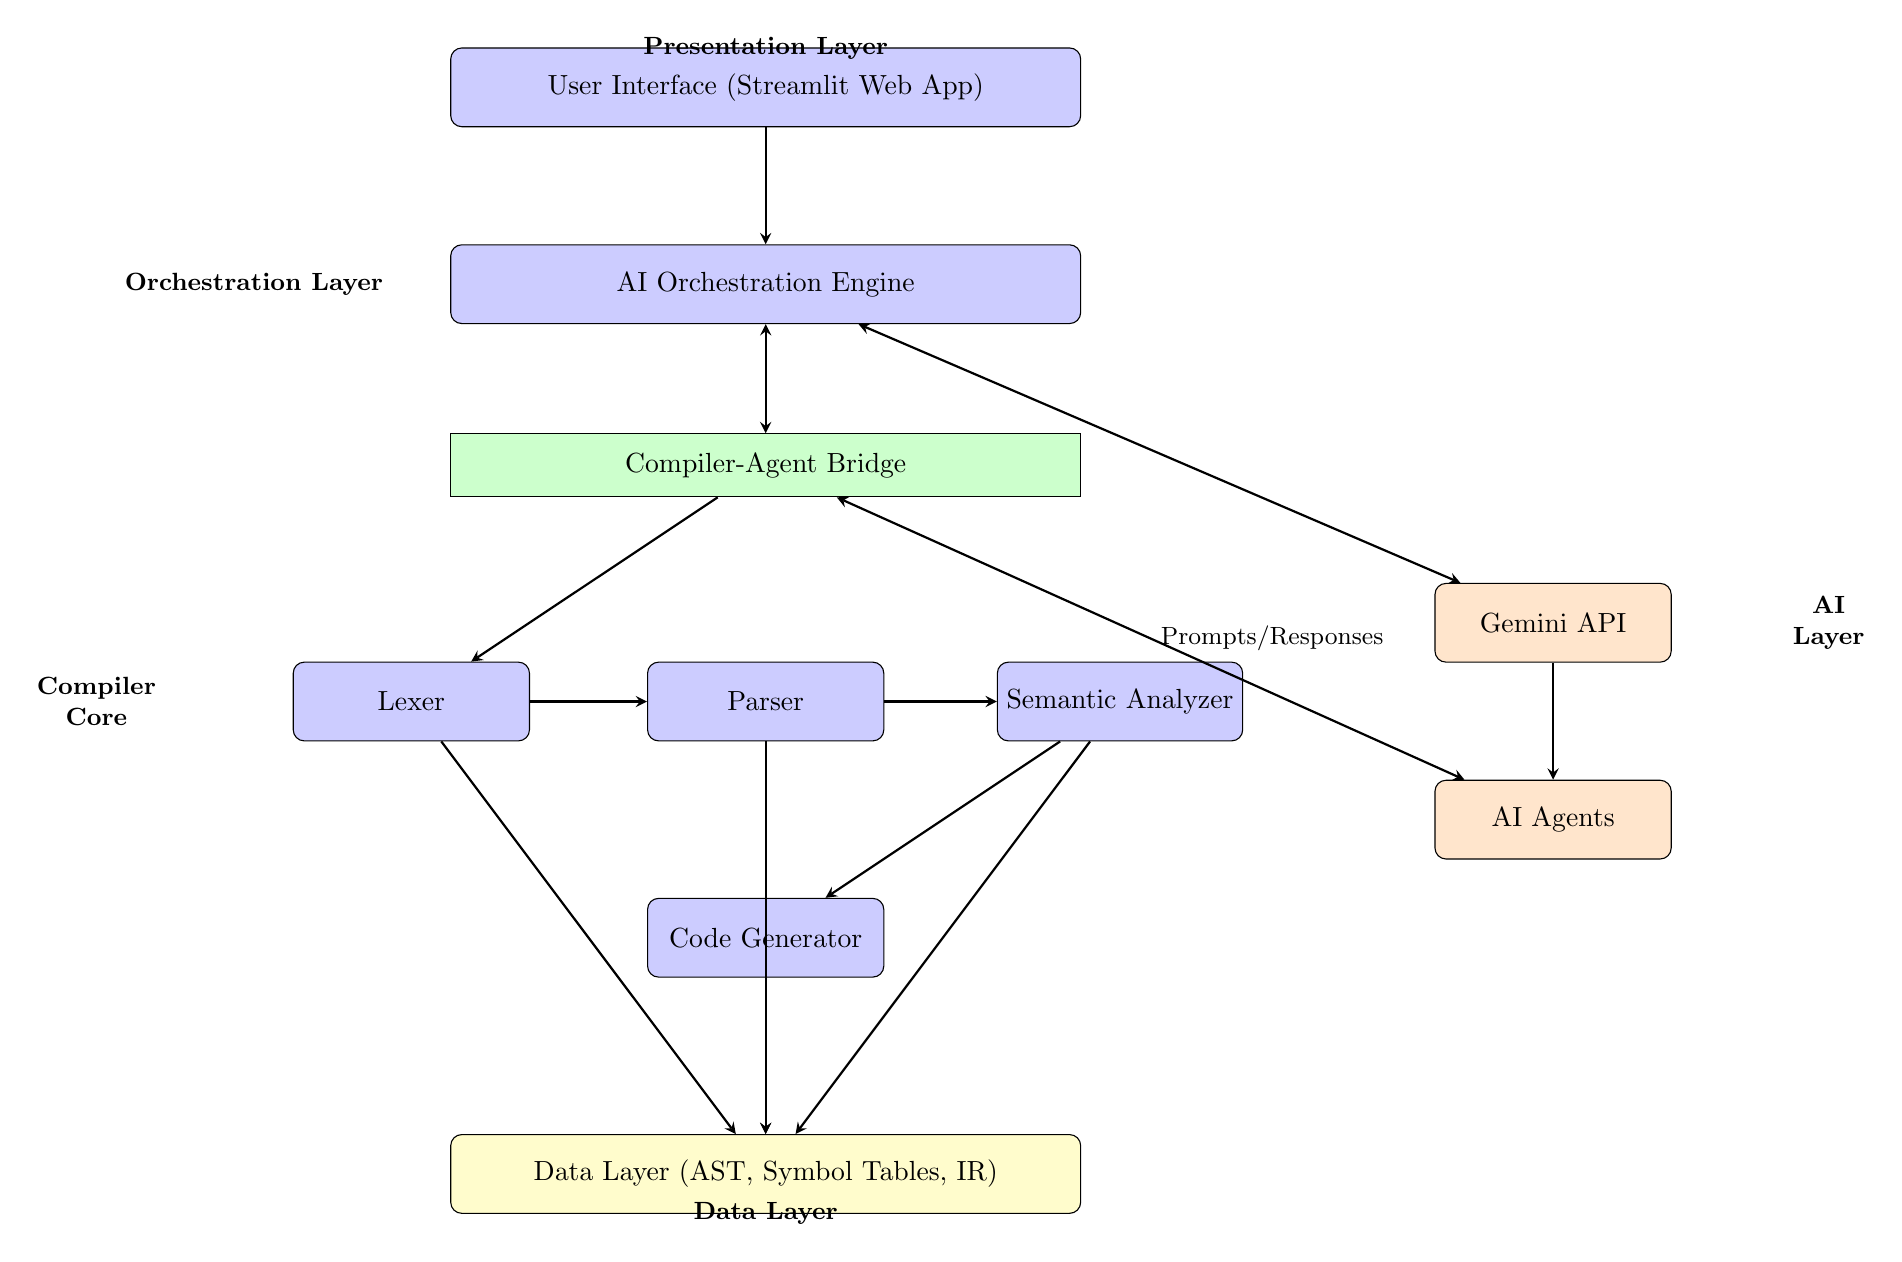
\begin{tikzpicture}[node distance=2cm]

% User Interface Layer
\node (ui) [component, minimum width=8cm] {User Interface (Streamlit Web App)};

% AI Orchestration Layer
\node (orchestrator) [component, below of=ui, yshift=-0.5cm, minimum width=8cm] {AI Orchestration Engine};
\node (bridge) [interface, below of=orchestrator, yshift=-0.3cm, minimum width=8cm] {Compiler-Agent Bridge};

% Compiler Core Layer
\node (lexer) [component, below of=bridge, yshift=-1cm, xshift=-4.5cm] {Lexer};
\node (parser) [component, right of=lexer, xshift=2.5cm] {Parser};
\node (semantic) [component, right of=parser, xshift=2.5cm] {Semantic Analyzer};
\node (codegen) [component, below of=parser, yshift=-1cm] {Code Generator};

% AI Agents Layer
\node (gemini) [component, fill=orange!20, right of=semantic, xshift=3.5cm, yshift=1cm] {Gemini API};
\node (agents) [component, fill=orange!20, below of=gemini, yshift=-0.5cm] {AI Agents};

% Data Layer
\node (data) [component, fill=yellow!20, below of=codegen, yshift=-1cm, minimum width=8cm] {Data Layer (AST, Symbol Tables, IR)};

% Arrows
\draw [arrow] (ui) -- (orchestrator);
\draw [bidiarrow] (orchestrator) -- (bridge);
\draw [arrow] (bridge) -- (lexer);
\draw [arrow] (lexer) -- (parser);
\draw [arrow] (parser) -- (semantic);
\draw [arrow] (semantic) -- (codegen);

\draw [bidiarrow] (orchestrator) -- (gemini);
\draw [arrow] (gemini) -- (agents);
\draw [bidiarrow] (agents) -- node[anchor=west, font=\small] {Prompts/Responses} (bridge);

\draw [arrow] (lexer) -- (data);
\draw [arrow] (parser) -- (data);
\draw [arrow] (semantic) -- (data);
\draw [arrow] (codegen) -- (data);

% Layer labels
\node[above of=ui, yshift=-1.5cm, font=\small\bfseries] {Presentation Layer};
\node[left of=orchestrator, xshift=-4.5cm, font=\small\bfseries] {Orchestration Layer};
\node[left of=lexer, xshift=-2cm, font=\small\bfseries, align=center] {Compiler\\Core};
\node[right of=gemini, xshift=1.5cm, font=\small\bfseries, align=center] {AI\\Layer};
\node[below of=data, yshift=1.5cm, font=\small\bfseries] {Data Layer};

\end{tikzpicture}
\caption{High-Level System Architecture}
\end{figure}

\section{Architectural Layers Details}

\subsection{3.1 Presentation Layer}

\textbf{Component:} Streamlit Web Application

\textbf{Responsibilities:}
\begin{itemize}[leftmargin=*]
    \item Accept user input (Mini-Python source code)
    \item Display compilation results, errors, and AI suggestions
    \item Provide conversational interface for user queries
    \item Visualize AST structures and compilation phases
    \item Show real-time compilation progress
\end{itemize}

\textbf{Key Features:}
\begin{itemize}[leftmargin=*]
    \item Code editor with syntax highlighting
    \item Phase-by-phase compilation visualization
    \item Error highlighting with line numbers
    \item AI chat interface for debugging assistance
    \item Export generated code and intermediate representations
\end{itemize}

\subsection{3.2 AI Orchestration Layer}

\textbf{Component:} AI Orchestration Engine

\textbf{Architecture:}

\begin{lstlisting}[language=Python, caption=Orchestration Engine Structure]
class AIOrchestrator:
    """Coordinates AI agents and compiler pipeline"""
    def __init__(self):
        self.bridge = CompilerAgentBridge()
        self.agent_manager = AgentManager()
        self.context_manager = ContextManager()
    
    def process_compilation(self, source_code):
        """Main compilation workflow with AI assistance"""
        # Phase 1: Lexical Analysis
        tokens = self.run_phase_with_ai_support(
            phase="lexer",
            input_data=source_code
        )
        
        # Phase 2: Parsing
        ast = self.run_phase_with_ai_support(
            phase="parser",
            input_data=tokens
        )
        
        # Phase 3: Semantic Analysis
        validated_ast = self.run_phase_with_ai_support(
            phase="semantic",
            input_data=ast
        )
        
        # Phase 4: Code Generation
        target_code = self.run_phase_with_ai_support(
            phase="codegen",
            input_data=validated_ast
        )
        
        return target_code
    
    def run_phase_with_ai_support(self, phase, input_data):
        """Execute compiler phase with AI assistance"""
        try:
            # Run compiler phase
            result = self.bridge.execute_phase(phase, input_data)
            return result
        except CompilationError as e:
            # AI intervention on errors
            suggestion = self.agent_manager.get_error_fix(
                phase=phase,
                error=e,
                context=self.context_manager.get_context()
            )
            return suggestion
\end{lstlisting}

\textbf{Responsibilities:}
\begin{itemize}[leftmargin=*]
    \item Manage compilation workflow across all phases
    \item Coordinate AI agent invocations at appropriate decision points
    \item Handle error recovery with AI assistance
    \item Maintain compilation context and state
    \item Provide explanations for compilation decisions
\end{itemize}

\subsection{3.3 Compiler-Agent Bridge}

\textbf{Critical Design Component:} This bridge serves as the interface between deterministic compiler components and non-deterministic AI agents.

\begin{figure}[h]
\centering
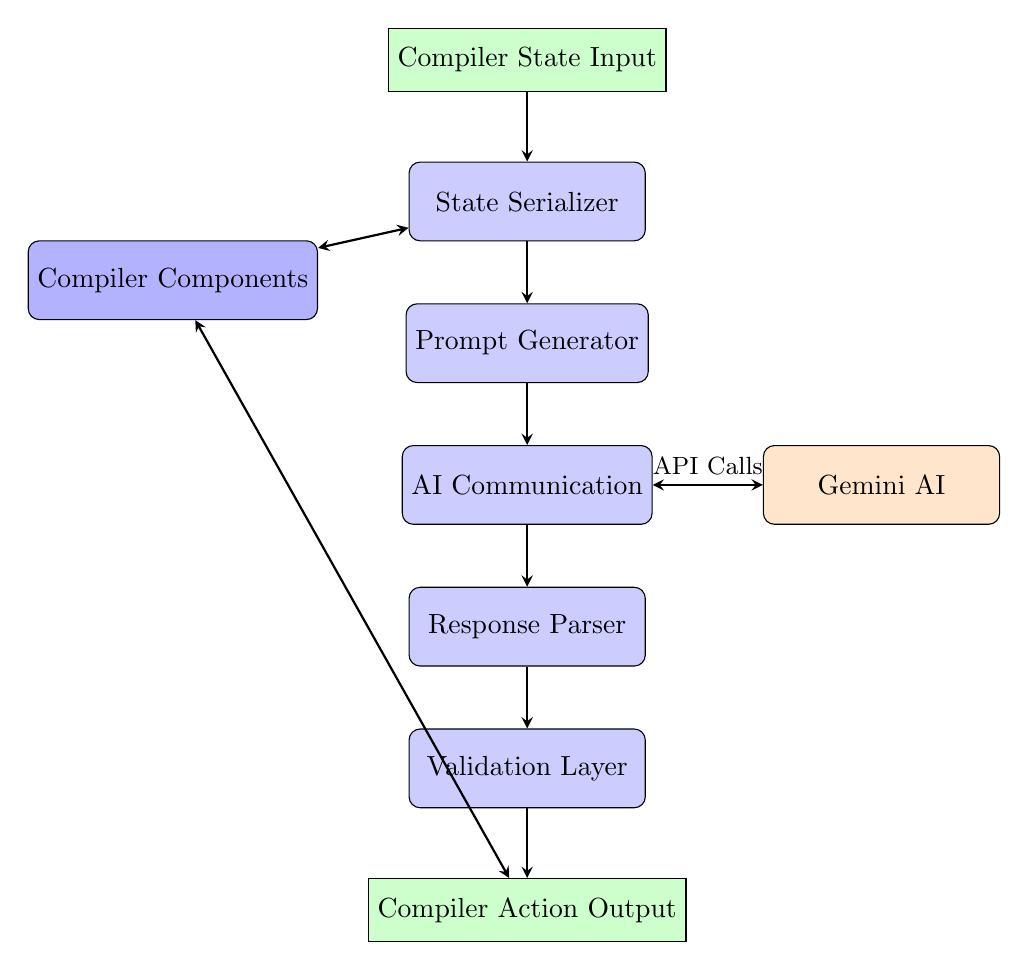
\begin{tikzpicture}[node distance=1.5cm]

% Bridge components
\node (input) [interface] {Compiler State Input};
\node (serializer) [component, below of=input, yshift=-0.3cm] {State Serializer};
\node (promptgen) [component, below of=serializer, yshift=-0.3cm] {Prompt Generator};
\node (aicomm) [component, below of=promptgen, yshift=-0.3cm] {AI Communication};
\node (responseparser) [component, below of=aicomm, yshift=-0.3cm] {Response Parser};
\node (validator) [component, below of=responseparser, yshift=-0.3cm] {Validation Layer};
\node (output) [interface, below of=validator, yshift=-0.3cm] {Compiler Action Output};

% External connections
\node (compiler) [component, fill=blue!30, left of=serializer, xshift=-3cm, yshift=-1cm] {Compiler Components};
\node (ai) [component, fill=orange!20, right of=aicomm, xshift=3cm] {Gemini AI};

% Arrows
\draw [arrow] (input) -- (serializer);
\draw [arrow] (serializer) -- (promptgen);
\draw [arrow] (promptgen) -- (aicomm);
\draw [arrow] (aicomm) -- (responseparser);
\draw [arrow] (responseparser) -- (validator);
\draw [arrow] (validator) -- (output);

\draw [bidiarrow] (compiler) -- (serializer);
\draw [bidiarrow] (compiler) -- (output);
\draw [bidiarrow] (aicomm) -- node[above, font=\small] {API Calls} (ai);

\end{tikzpicture}
\caption{Compiler-Agent Bridge Architecture}
\end{figure}

\textbf{Bridge Responsibilities:}

\begin{enumerate}
    \item \textbf{State Serialization:}
    \begin{itemize}[leftmargin=*]
        \item Convert AST to JSON representation
        \item Serialize symbol tables and type information
        \item Package error contexts with relevant source code
    \end{itemize}
    
    \item \textbf{Prompt Engineering:}
    \begin{itemize}[leftmargin=*]
        \item Inject Mini-Python grammar into prompts
        \item Provide compilation phase context
        \item Include relevant examples from knowledge base
        \item Format error information for AI understanding
    \end{itemize}
    
    \item \textbf{Response Parsing:}
    \begin{itemize}[leftmargin=*]
        \item Extract structured data from AI natural language responses
        \item Parse code suggestions and corrections
        \item Validate AI-generated code against grammar
    \end{itemize}
    
    \item \textbf{Validation \& Safety:}
    \begin{itemize}[leftmargin=*]
        \item Verify AI suggestions don't introduce security issues
        \item Validate generated code maintains semantic correctness
        \item Ensure AI responses align with compiler state
    \end{itemize}
\end{enumerate}

\textbf{Implementation Example:}

\begin{lstlisting}[language=Python, caption=Compiler-Agent Bridge Core Methods]
class CompilerAgentBridge:
    """Bridge between compiler and AI agents"""
    
    def serialize_compiler_state(self, phase, data, error=None):
        """Convert compiler state to AI-friendly format"""
        state = {
            "phase": phase,
            "timestamp": datetime.now().isoformat(),
            "grammar": self.load_grammar(),
            "data": self._serialize_data(data),
            "error": self._serialize_error(error) if error else None
        }
        return json.dumps(state, indent=2)
    
    def generate_prompt(self, task_type, context):
        """Generate contextual prompt for AI"""
        templates = {
            "error_fix": """You are assisting with {phase} phase of compilation.
            
Grammar:
{grammar}

Current State:
{state}

Error:
{error}

Please suggest a fix and explain the issue.""",
            
            "optimization": """Analyze this {phase} output for optimization opportunities.
            
Current Implementation:
{implementation}

Suggest improvements while maintaining correctness."""
        }
        
        template = templates[task_type]
        return template.format(**context)
    
    def parse_ai_response(self, response, expected_format):
        """Extract structured data from AI response"""
        # Use regex and parsing to extract code blocks
        code_blocks = self._extract_code_blocks(response)
        explanation = self._extract_explanation(response)
        
        # Validate against expected format
        validated = self.validate_response(code_blocks, expected_format)
        
        return {
            "code": validated,
            "explanation": explanation,
            "confidence": self._estimate_confidence(response)
        }
\end{lstlisting}

\subsection{3.4 Compiler Core Layer}

\textbf{Traditional Compiler Pipeline:}

The compiler core implements a standard multi-phase compilation pipeline:

\begin{table}[h]
\centering
\begin{tabularx}{\textwidth}{|l|X|X|}
\hline
\rowcolor{blue!10}
\textbf{Component} & \textbf{Input} & \textbf{Output} \\
\hline
Lexer & Source code string & Token stream \\
\hline
Parser & Token stream & Abstract Syntax Tree (AST) \\
\hline
Semantic Analyzer & AST & Validated AST + Symbol Table \\
\hline
Code Generator & Validated AST & Target code (Python bytecode/C++) \\
\hline
\end{tabularx}
\caption{Compiler Pipeline Phases}
\end{table}

\textbf{Class Hierarchy:}

\begin{lstlisting}[language=Python, caption=Compiler Component Interfaces]
class CompilerPhase(ABC):
    """Abstract base for all compiler phases"""
    @abstractmethod
    def process(self, input_data):
        """Process input and return output"""
        pass
    
    @abstractmethod
    def get_errors(self):
        """Return list of errors encountered"""
        pass

class Lexer(CompilerPhase):
    """Lexical analysis - source to tokens"""
    def process(self, source_code: str) -> List[Token]:
        return self.tokenize(source_code)

class Parser(CompilerPhase):
    """Syntax analysis - tokens to AST"""
    def process(self, tokens: List[Token]) -> AST:
        return self.parse(tokens)

class SemanticAnalyzer(CompilerPhase):
    """Semantic analysis - validate AST"""
    def process(self, ast: AST) -> Tuple[AST, SymbolTable]:
        return self.analyze(ast)

class CodeGenerator(CompilerPhase):
    """Code generation - AST to target code"""
    def process(self, ast: AST) -> str:
        return self.generate(ast)
\end{lstlisting}

\subsection{3.5 AI Agent Layer}

\textbf{Specialized AI Agents:}

\begin{table}[h]
\centering
\begin{tabularx}{\textwidth}{|l|X|X|}
\hline
\rowcolor{blue!10}
\textbf{Agent} & \textbf{Purpose} & \textbf{Activation Trigger} \\
\hline
Error Diagnostic Agent & Explain compilation errors to users & Any compiler error \\
\hline
Fix Suggestion Agent & Suggest code fixes & Syntax or semantic errors \\
\hline
Optimization Agent & Recommend code improvements & User request or completion \\
\hline
Explanation Agent & Explain compilation process & User query \\
\hline
Code Review Agent & Review generated code quality & Post-generation \\
\hline
\end{tabularx}
\caption{AI Agent Specializations}
\end{table}

\subsection{3.6 Data Layer}

\textbf{Persistent and Transient Data:}

\begin{itemize}[leftmargin=*]
    \item \textbf{AST Storage:} In-memory representation during compilation
    \item \textbf{Symbol Tables:} Scope-based symbol tracking
    \item \textbf{Intermediate Representation (IR):} Three-address code or LLVM IR
    \item \textbf{Error Logs:} Compilation errors with context
    \item \textbf{AI Interaction History:} Previous queries and responses for context
\end{itemize}

\section{Data Flow Architecture}

\subsection{4.1 Compilation Data Flow}

\begin{figure}[h]
\centering
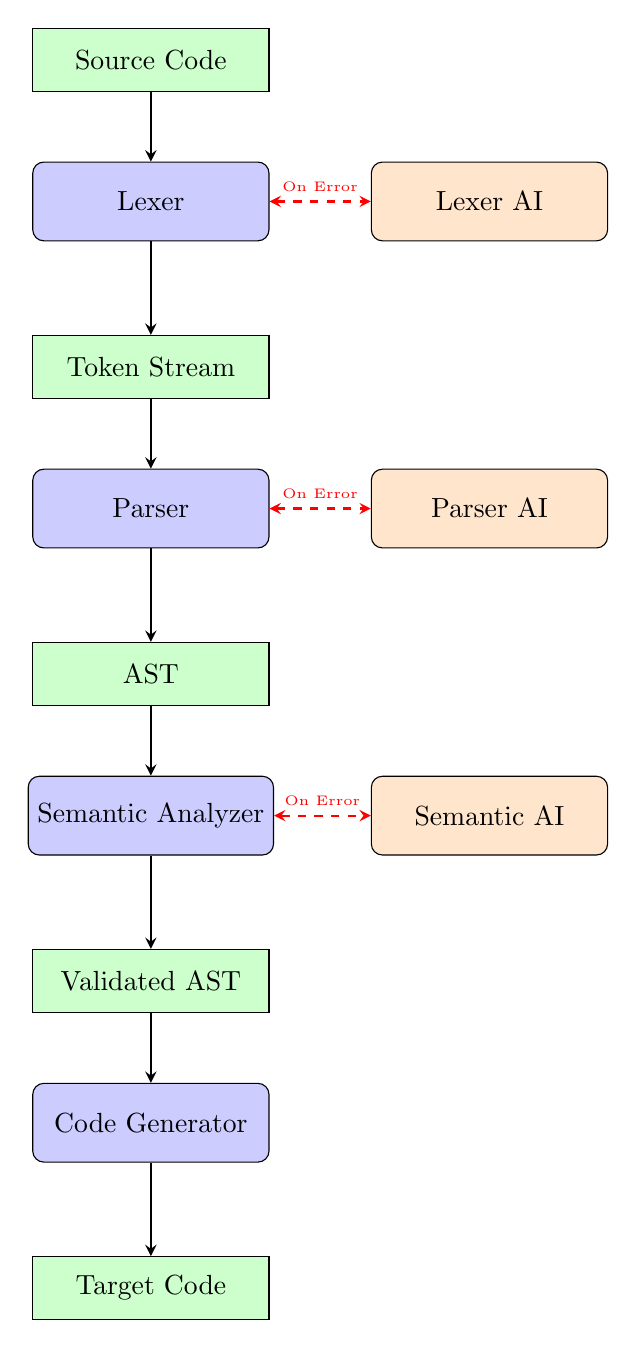
\begin{tikzpicture}[node distance=1.8cm, auto]

\node (source) [interface] {Source Code};
\node (lexer) [component, below of=source] {Lexer};
\node (tokens) [interface, below of=lexer, yshift=-0.3cm] {Token Stream};
\node (parser) [component, below of=tokens] {Parser};
\node (ast) [interface, below of=parser, yshift=-0.3cm] {AST};
\node (semantic) [component, below of=ast] {Semantic Analyzer};
\node (validated) [interface, below of=semantic, yshift=-0.3cm] {Validated AST};
\node (codegen) [component, below of=validated] {Code Generator};
\node (output) [interface, below of=codegen, yshift=-0.3cm] {Target Code};

% AI intervention points
\node (ai1) [component, fill=orange!20, right of=lexer, xshift=2.5cm] {Lexer AI};
\node (ai2) [component, fill=orange!20, right of=parser, xshift=2.5cm] {Parser AI};
\node (ai3) [component, fill=orange!20, right of=semantic, xshift=2.5cm] {Semantic AI};

\draw [arrow] (source) -- (lexer);
\draw [arrow] (lexer) -- (tokens);
\draw [arrow] (tokens) -- (parser);
\draw [arrow] (parser) -- (ast);
\draw [arrow] (ast) -- (semantic);
\draw [arrow] (semantic) -- (validated);
\draw [arrow] (validated) -- (codegen);
\draw [arrow] (codegen) -- (output);

\draw [bidiarrow, dashed, color=red] (lexer) -- node[above, font=\tiny] {On Error} (ai1);
\draw [bidiarrow, dashed, color=red] (parser) -- node[above, font=\tiny] {On Error} (ai2);
\draw [bidiarrow, dashed, color=red] (semantic) -- node[above, font=\tiny] {On Error} (ai3);

\end{tikzpicture}
\caption{Compilation Data Flow with AI Intervention Points}
\end{figure}

\section{Technical Decisions \& Justifications}

\subsection{5.1 Technology Stack}

\begin{table}[h]
\centering
\begin{tabularx}{\textwidth}{|l|l|X|}
\hline
\rowcolor{blue!10}
\textbf{Category} & \textbf{Technology} & \textbf{Justification} \\
\hline
Language & Python 3.10+ & Rapid development, rich ecosystem, AI/ML library support \\
\hline
AI Model & Gemini-1.5-Pro & Superior code understanding, large context window (1M tokens) \\
\hline
Frontend & Streamlit & Rapid prototyping, built-in widgets, real-time updates \\
\hline
Testing & pytest + coverage & Industry standard, extensive plugin ecosystem \\
\hline
AST Manipulation & dataclasses & Clean, immutable node definitions \\
\hline
Serialization & JSON & Human-readable, AI-friendly format \\
\hline
\end{tabularx}
\caption{Technology Stack Decisions}
\end{table}

\subsection{5.2 Design Patterns Applied}

\begin{enumerate}
    \item \textbf{Visitor Pattern:} AST traversal for semantic analysis and code generation
    \item \textbf{Bridge Pattern:} Compiler-Agent Bridge decouples compiler from AI
    \item \textbf{Factory Pattern:} Token and AST node creation
    \item \textbf{Strategy Pattern:} Different code generation strategies (Python/C++)
    \item \textbf{Observer Pattern:} Compilation progress notifications to UI
    \item \textbf{Chain of Responsibility:} Error handling across compilation phases
\end{enumerate}

\section{Quality Attributes}

\subsection{6.1 Non-Functional Requirements}

\begin{table}[h]
\centering
\begin{tabularx}{\textwidth}{|l|X|X|}
\hline
\rowcolor{blue!10}
\textbf{Attribute} & \textbf{Requirement} & \textbf{Implementation Strategy} \\
\hline
Performance & Compile 100-line program in < 2 seconds & Optimized regex, efficient AST structures \\
\hline
Reliability & 95\%+ test coverage & Comprehensive unit and integration tests \\
\hline
Maintainability & Modular design & Clear interfaces, documentation \\
\hline
Extensibility & Easy to add new language features & Plugin architecture for grammar extensions \\
\hline
Usability & Intuitive error messages & AI-enhanced explanations \\
\hline
\end{tabularx}
\caption{Quality Attributes}
\end{table}

\section{Risks \& Mitigation Strategies}

\begin{table}[h]
\centering
\begin{tabularx}{\textwidth}{|l|X|X|}
\hline
\rowcolor{blue!10}
\textbf{Risk} & \textbf{Impact} & \textbf{Mitigation} \\
\hline
AI API failures & High - breaks assistance & Graceful degradation, caching responses \\
\hline
Incorrect AI suggestions & Medium - user confusion & Validation layer, confidence scoring \\
\hline
Performance issues & Medium - poor UX & Async processing, progress indicators \\
\hline
Complex grammar & High - limits functionality & Iterative development, start simple \\
\hline
\end{tabularx}
\caption{Risk Management}
\end{table}

\section{Deliverables}

\textbf{Architecture Documentation:}
\begin{itemize}[leftmargin=*]
    \item System Architecture Specification (45 pages)
    \item 5 UML diagrams (System overview, Component, Data flow, Sequence, Class)
    \item Interface definitions for all components
    \item Data model specifications
\end{itemize}

\textbf{Technical Specifications:}
\begin{itemize}[leftmargin=*]
    \item Compiler-Agent Bridge API specification
    \item AI prompt templates for each compilation phase
    \item Error handling workflows
    \item Data serialization formats (AST to JSON schema)
\end{itemize}

\section{Metrics}

\begin{table}[h]
\centering
\begin{tabularx}{\textwidth}{|l|c|c|X|}
\hline
\rowcolor{blue!10}
\textbf{Metric} & \textbf{Target} & \textbf{Actual} & \textbf{Status} \\
\hline
Architecture Completeness & 100\% & 100\% & \statusgood{Complete} \\
\hline
UML Diagrams & 5 & 5 & \statusgood{Complete} \\
\hline
Component Specifications & 6 & 6 & \statusgood{Complete} \\
\hline
Documentation Pages & 40+ & 45 & \statusgood{Exceeded} \\
\hline
Schedule Adherence & On Track & On Track & \statusgood{On Track} \\
\hline
\end{tabularx}
\caption{Week 4 Performance Metrics}
\end{table}

\section{Next Week Preview}

\textbf{Focus:} Lexer Implementation (Week 5)

\textbf{Planned Activities:}
\begin{itemize}[leftmargin=*]
    \item Implement Token and TokenType classes based on architecture
    \item Build regex-based tokenization engine
    \item Implement Python indentation handling (INDENT/DEDENT tokens)
    \item Create comprehensive lexer test suite (45+ tests)
    \item Integrate lexer with basic UI for testing
    \item Document lexer implementation
\end{itemize}

\textbf{Success Criteria:}
\begin{itemize}[leftmargin=*]
    \item Lexer correctly tokenizes all Mini-Python constructs
    \item 95\%+ test coverage for lexer component
    \item Indentation handling matches Python's behavior
    \item Detailed error reporting with line/column information
\end{itemize}

\section{Conclusion}

Week 4 successfully established a comprehensive, professional system architecture that bridges traditional compiler design with modern AI capabilities. The modular, layered approach ensures each component can be developed independently while maintaining clear interfaces and data contracts.

The Compiler-Agent Bridge serves as the critical innovation, enabling seamless integration between deterministic compilation phases and AI-powered assistance without compromising the correctness of the traditional compiler pipeline.

All architectural deliverables were completed on schedule with extensive documentation. The project is well-positioned to begin implementation in Week 5 with a solid technical foundation.

\vspace{5mm}
\noindent\textbf{Prepared by:} Project Team \\
\textbf{Reporting Date:} Week 4 Completion \\
\textbf{Next Review:} Week 5 Report \\
\textbf{Documentation:} 45 pages of architectural specifications

\end{document}